\chapter{引言}
\label{cha:intro}

\section{研究背景}
近年来,随着智能手机的普及以及移动互联网的快速发展,基于移动互联网以及用户位置的应用正呈现井喷式的增长,而因为LTE网络的普及以及5G的即将到来,智能终端将与日俱增,与之对应的高精度定位也将变得更加重要,比如自动驾驶中的高精度定位。除此之外,定位技术还广泛应用于商业广告、购物消费、医疗保健、险情救援等诸多领域,从传统的手机定位导航到近几年兴起的网约车以及共享单车都是用户定位改变人们生活的典型范例。正因为定位是众多应用的基础必需模块,定位问题及其后续服务一直是学术界的研究热点。

\subsection{定位问题}

在开阔的室外环境中,以 GPS(Global  Positioning System)和北斗为代表的卫星定位系统已经能够实现准确的定位~\cite{xiao2016survey},这也是目前定位算法最成功的的实现之一。然而,卫星定位仍然存在一些目前无法妥善解决的问题。首先,卫星定位的结果只能在终端(client)解算得到,因此服务端(server)只能依靠用户上传自己的位置获得其定位。这在某些场景下是不适用的,比如对非法电台的定位。其次,卫星定位需要用户终端硬件支持卫星信号,这不仅增加手机制造的成本,而且对于不支持卫星定位的老旧手机无法定位。最后,由于卫星信号强度弱使得其抗干扰和遮挡能力弱,因此卫星定位在室内和高楼遮挡较多的市区无法准确定位。

目前基于非卫星信号的定位主要应用于室内定位(Indoor Localization)和无线传感器网络(Wireless Sensor Network)定位。在这些场景下,多种特征被用于定位,包括接收信号强度(Received Signal Strength, RSS)~\cite{vaghefi2013cooperative, jackson2011received, liu2006analysis, bahl2000radar}、信号到达时间(time-of-arrival)~\cite{guvenc2009survey}、到达时间差(time-difference-of-arrival)~\cite{catovic2004cramer}和到达角(angle-of-arrival)~\cite{cong2002hybrid}。其中,到达时间需要终端和无线接入点(Wireless Access Point, WAP)时间同步,到达时间差一般是无线电信号和另一个慢速传播信号(比如超声波)的传播时间差因此需要额外设备,到达角需要天线阵列从而提高了该方法的成本和能耗。只有基于RSS的方法不需要额外的硬件因为信号强度是实现通信的最基本要求。此外,美国国家通讯委员会于2005年提出了E911紧急定位要求:定位精度在67\%的概率下处于50m~100m区间,以95\%的概率处于150m~300m区间~\cite{junglas2008location}。只有基于RSS的定位算法可以在当前条件下可以对所有手机定位。因此我们的研究将专注于基于RSS的定位算法。

\subsection{广告投放问题}

在解决定位问题获得用户位置后,如何更好的使用也是一个有意义的课题。其中,基于用户定位的信息和广告投放吸引了越来越多的关注。“2016年网络广告市场规模已达2902.7亿元, 其中移动网络广告超过60\%”~\cite{赵杨2018基于机器学习混合算法的},将用户位置信息应用于移动网络广告使得广告投放更精准是一个重要的课题。保量推荐广告(Guaranteed Delivery Advertisement)是互联网企业的主要收入来源之一~\cite{korula2016optimizing, mcafee2013maximally},广告主事先设定好广告量和投放时长,平台则是确保广告在结束投放之前获得足够的投放量的条件下,获得尽量好的投放效果(比如点击率,转化率等)。本文将研究基于用户定位的保量推荐算法。

每次页面访问(Page  View, PV)都会携带候选投放广告以及预测出的该用户对于这些广告的打分,我们将在候选广告中选取一个或几个广告投放给该用户或者不投放。在用户流中选择用户投放广告来最大化总的用户分数且保证曝光量并不是一件显而易见的事,因为决定投放哪条广告必须在秒量级的时间内决定,因此不可能将所有访问请求累积起来然后从中选几个最优的投放。一种最简单的实现则是针对每次访问,选择分数最高的广告,若分数最高的广告投放量已满则选择次高,以此类推。因为如下缺点,现实中这种实现方式并不适用:
\begin{itemize}
	\item 高质量广告即几乎所有用户对其打分都高的广告会快速投放完毕而低质量广告甚至可能无法保证曝光量。因为平稳投放也是我们的一个次要目标,所以该方法不适用;
	\item 该方案的投放结果与最优结果相去甚远。例如表\ref{tab:eoa}所示,有3次访问和2个广告,每个广告的投放量都是1。显然,最优投放策略应该是广告1 $\rightarrow$ PV 1,广告2 $\rightarrow$ PV 3,该策略总分是1.2。然而上文的贪心法策略是广告1 $\rightarrow$ PV 2,广告2 $\rightarrow$ PV 1,总分只有0.7。
\end{itemize}
\begin{table}[htb]
	\centering
	\caption{广告投放举例}
	\label{tab:eoa}
	\begin{tabular}{ccc}
		\toprule
		分数 & 广告 $1$ & 广告 $2$ \\
		\midrule
		PV $1$ & $0.5$ & $0.6$ \\
		\midrule
		PV $2$ & $0.1$ & $0.2$ \\
		\midrule
		PV $3$ & $0.3$ & $0.7$ \\
		\bottomrule
	\end{tabular}
\end{table}
为了解决上述问题,我们提出了一种保量推荐下的最优广告投放算法

快手(Kwai)作为世界上最大的短视频平台之一,为视频作者提供名为“粉丝头条”的服务来帮助他们推广自己的作品,是一种保量推荐广告。粉丝头条的购买者需设定期望的曝光量(即该视频出现在他人视频页面上的数量)和投放时长,我们在确保曝光量的同时使得投放结束后用户获得最多的涨粉数(即关注量或订阅量)增加。快手的视频页面分为“关注”、“发现”和“同城”三栏,其中同城页的视频按照访问者与视频作者之间的距离筛选视频。我们的算法将部署在快手同城页粉丝头条服务中。

\begin{figure}
	\centering
	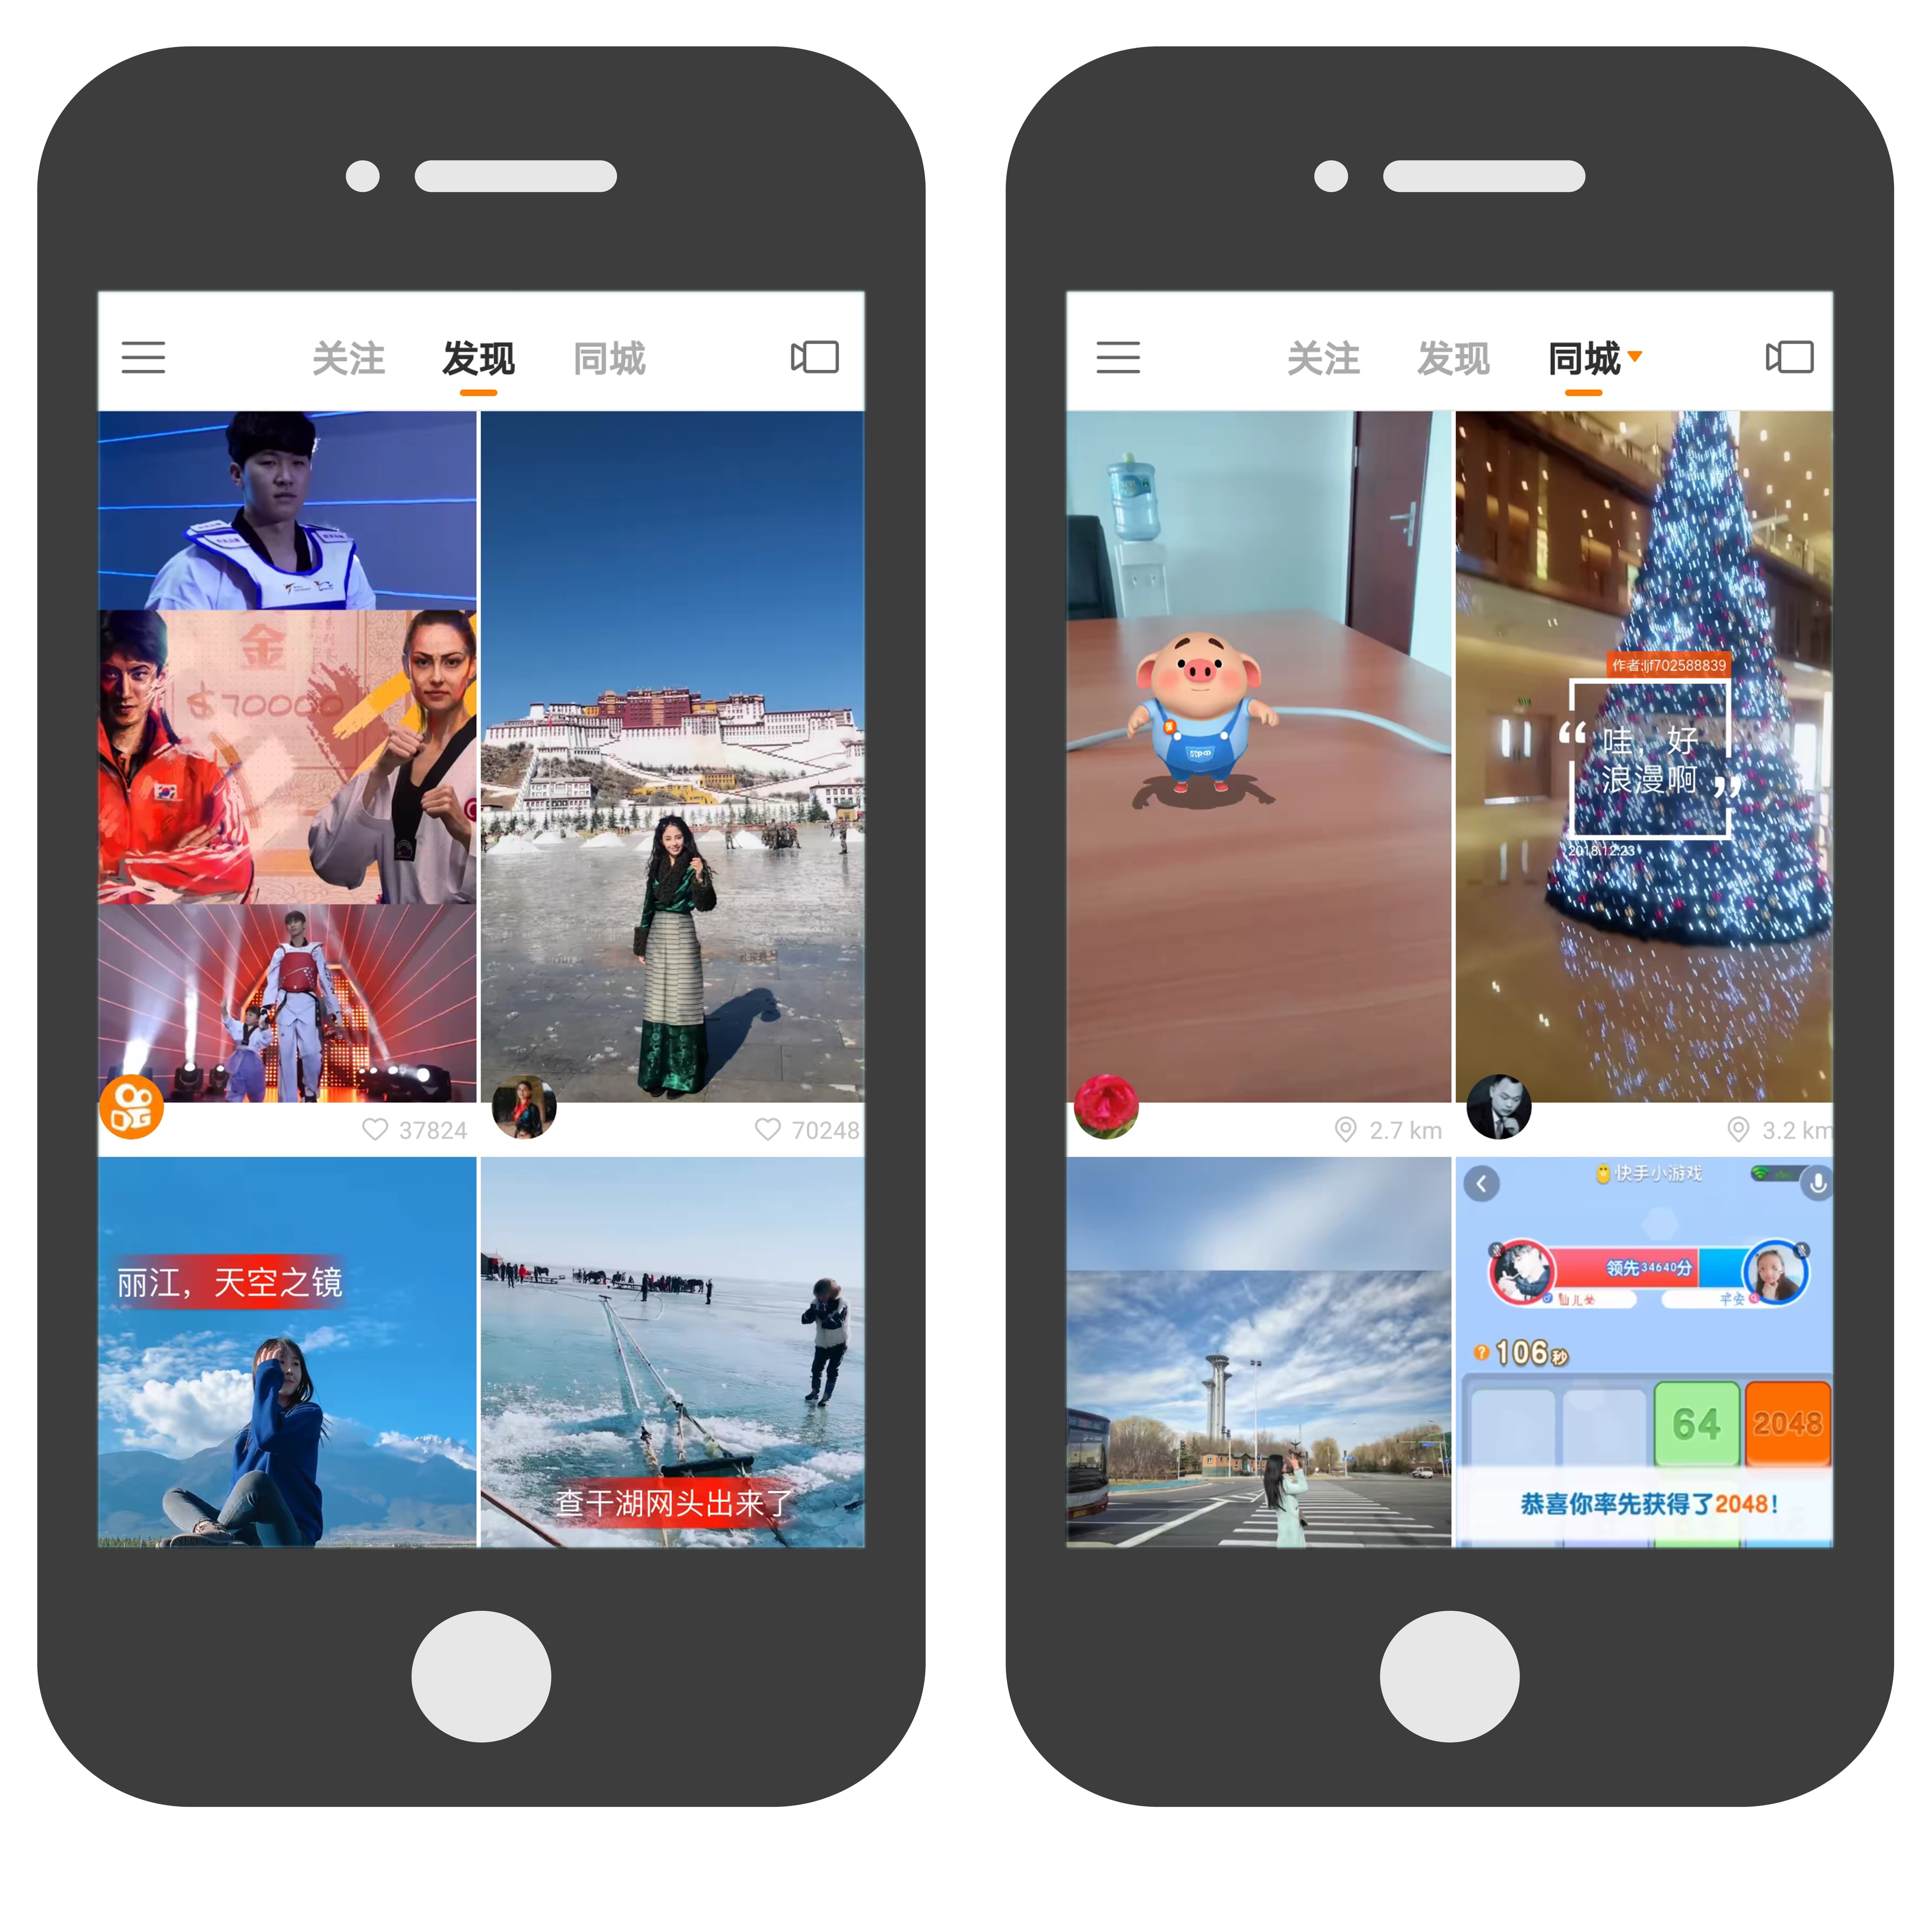
\includegraphics[width=0.5\textwidth]{Kwai.jpg}
	\caption{如图所示为快手发现页和同城页的页面设计,本文主要关注右子图即同城页。在同城页展现给用户的视频会先根据用户与视频作者之间的距离筛选。}
	\label{fig:kwai}
\end{figure}

\section{定位与广告投放算法的研究现状}
\label{sec:first}

\subsection{定位方法的研究现状}

上一小节中我们根据定位所采用的信号特征将定位算法分类,其中只有基于RSS的方法不需要额外硬件兼容现有通信设备,因此这里仅分析研究基于RSS的定位算法。

我们可以按照定位目标是信号发射源还是接收端来分类算法。当用户作为信号发射源时,他的位置是由分散在其周围的结点根据RSS联合计算获得的,若用户想获知自己的位置需要从服务器下载。与之对应的,当用户作为信号接收端时,通过汇总信号解算在终端本地解算获得其位置信息或者上传到服务器解算。非法电台定位场景下的算法就是前者,而卫星定位是后者的典型代表。

此外,在基于RSS的定位中,如果按照定位算法的求解方式分类,还可以将算法分为基于求解优化问题或是基于模式识别。前者需要对信号传输建模,设计误差函数后找出定位位置值使其最小。后者需要大量采集当地信号作为指纹(Fingerprint)/数据库(Database),在定位时设计算法将信号与指纹/数据库进行匹配得到位置,这种方法又被称为“指纹定位”(Fingerprint Localization)或“数据库相关算法”。前者不需要大量的事先数据采集工作且泛化能力强,但是信道建模是一个难点,因为简单模型不能反应真实情况会降低定位准确性,而复杂模型又会提高计算复杂度。同时,前者的误差函数一般都是非凸的从而导致求解困难。反之,后者不需要复杂的建模工作而且一般来说定位精度更高,不过需要大量的数据采集而且一旦在一个新的区域定位就得重新采集数据。发射源定位多采用前者因为用户作为发射源时其发射功率无法保证恒定,而且一旦用户移动,所有位置的RSS都会变化。接收端定位则二者兼有实现实例,但在室内定位中多采用指纹定位,因为定位精度高且定位区域小,数据采集简单。

接下来我们将分别从基于求解优化问题定位和指纹定位两个方面综述。

\subsubsection{基于求解优化问题的定位}

使用该方法定位有一个最基本假设即发射源功率是恒定的,一般来说这个假设都可以满足。该方法可以被分为两类:有锚点(Anchor Point)和无锚点,其中锚点是一个距离发射源距离已知的点。在无线传感器网络中锚点很常见,但是在某些场景下这个假设过强,比如定位非法电台。在后续讨论中我们只关心无锚点的情况。

在无锚点的情况下,最大似然法(Maximum Likelihood, ML)是最常用的估计器和基准(Baseline)。许多其他基于ML的估计器被提出了,但是无论是半正定规划还是线性最小二乘(Linear Least Square, LLS)都不能取得比ML更低的误差~\cite{jackson2011received}。他们的改进点在于将原来的非凸优化转化为凸优化问题,虽然改变后可以保证取得最优解从而提高了求解效率,但是改变目标函数也使得新问题的最优解依然不是原问题的最优解。

两种基于LLS的算法被提出~\cite{wang2011near},其推导过程表明每两个信号接收点可以形成一个发射源坐落在其上的圆。但是,作者之后提出了两种LLS解法而没有在针对这个现象深入研究。我们将提出一种算法,基于这些圆的几何意义定位发射源,即找到一个点到所有圆边缘的距离之和最小。另一种基于圆定位发射源的算法已经被提出~\cite{liu2006analysis},但是这篇文章的应用场景是有锚点的,而且克拉美罗下界(Cram\'{e}r-Rao Lower Bound, CRLB)没有被分析。CRLB是估计器误差的理论下界。

\subsubsection{指纹定位}

如本节开篇所述,指纹定位是对基于模式识别的定位算法的别称。指纹定位能够比传统算法表现更好是因为后者需要视线内通信~\cite{gentile2012geolocation},而这个条件对于城市内和室内定位过于严苛。指纹定位由线下和线上两部分组成。线下部分组件数据库,数据是由物理空间中的坐标和信号空间中的RSS结对组成。线上部分则根据输入的RSS计算定位。

指纹定位有很多种实现方式,从K近邻(K Nearest Neighbors, KNN)到支持向量机(Support Vector Machine, SVM)和深度学习(Deep Learning, DL)。因为其计算成本低且定位效果好,KNN及其衍生算法在指纹定位中被广泛使用~\cite{xia2017indoor}。加权KNN(Weighted-KNN)是KNN的诸多衍生算法中的一个,它的定位精度优于经典KNN~\cite{yen2017modified}。

除了代表近邻数的参数$k$,距离度量方式也是KNN中的一个重要参数。只有一些常用的度量方式被经常采用和比较定位效果,比如欧氏距离(Euclidean Distance)、曼哈顿距离(Manhattan Distance)和余弦相似度(Cosine Similarity)。目前已经有一些文章针对这些常用度量方式进行比较。当曼哈顿距离与欧氏距离和谷本距离(Tanimoto Distance)比较时,曼哈顿距离定位精度更高~\cite{marques2012combining}。在某些情况下,余弦相似度也会取得比欧氏距离更小的误差~\cite{han2015cosine}。但是,上述所有度量方式都给予大RSS和小RSS相同的权重,但这可能并不是一种理想的选择。指数变换法被提出来解决这个问题~\cite{torres2015comprehensive}。但是变换中参数对结果的影响没有被分析,相关的实验会在本文中开展。

切线距离(Tangent Distance)最早被提出以解决手写数字识别问题~\cite{simard1998transformation},它是对于流形(Manifold)之间距离的局部线性近似。流形是机器学习领域中的经典假设,即高维输入数据一般都居于或邻近低维流形上~\cite{roweis2000nonlinear},并且数据的微小扰动会形成流形。在这种情况下,两点之间的真实距离并不是简单的距离而是这两个点所在的不同流形之间的距离。在原文中,切线距离是基于欧氏距离的但是在我们的实验中欧氏距离表型并不如曼哈顿距离。因此我们将提出一种基于曼哈顿距离的切线距离来提高定位精度。

\subsection{广告推送算法的研究现状}

预算广告(Budget Advertising)在过去几年正在吸引越来越多的关注。快手的粉丝头条广告和目标广告(Target Advertising)~\cite{xu2015smart}以及搜索广告(Search Advertising)~\cite{mehta2005adwords}有很多相似之处。广告主在目标广告中设定一些目标用户的属性而在搜索广告中设定一些在线搜索关键字。我们的场景与二者的不同之处在于我们的约束是实际曝光量最好等于期望曝光量,而后两者的约束是广告消费金额不能超过广告主的预算,同时几乎所有的目标广告和搜索广告的目标都是最大化收入或者平稳投放,因此这些算法需要修改以适应我们的问题。Feldman et al. ~\cite{feldman2010online}证明了基于训练的对偶法(primal-dual)的有效性,但是因为文中的目标函数采用的线性函数,导致在线投放机制是启发式的。Devanur 和 Hayes~\cite{devanur2009adwords} 提出了一种平滑的线性规划(Linear Programming, LP)来避免竞价时出现相同竞价权重的问题。但是,该方法目标是最大化收入,而我们的目标是最大化点击率(Click-Through Rate, CTR)或者关注率(Follow Rate, FTR)。此外,他们的约束是广告平台从广告主的收费不能超过广告主的预算,不同于我们的实际曝光量最好和期望曝光量相等。针对该问题的解决,类似的公式曾被 Turner 提出过~\cite{turner2012planning},他的目标函数是二次函数且是等式约束。但是求解过程引入了除法操作,这在我们的算法实践中可能会造成严重问题,因为用户对视频的打分在 $10^{-5}$ 到 $10^{-2}$ 范围内变化,所以分数上的微小变化将会引起倒数的剧烈变化,即该解法使得问题病态。最后,实时竞价广告(Real-Time Bidding Advertising)和预算广告也有很多相似之处,Chen et al.~\cite{chen2011real} 提出了一种类似的基于LP的算法。

此外,一些研究分析了LP算法的对最优解的逼近程度。Devanur et al.~\cite{devanur2011near} 证明了在独立同分布的情况下,算法结果和最优解之比为 $1-O(\epsilon)$,其中 $\epsilon$ 是一个常数。深入的研究证明即使分布随时间变化,这个比例仍然能够达到 $1-\frac{1}{\sqrt{k+3}}$,其中 $k$ 代表最小容量~\cite{alaei2012online}。

我们的算法要部署在快手的商业化平台上,而快手的日均访问量是百亿级别的,因此除了广告投放效果之外,算法的计算时间和响应时间也是至关重要的。为了实现从理论到实践的过渡,有三大类实现方式:贪心法,启发式算法和凸优化。
\begin{itemize}
	\item Karande et al.~\cite{karande2013optimizing} 提供了一种快速贪心算法并且他们也把优化CTR纳入了考虑范围。但是贪心法的问题是没有不考虑到广告之间的互相影响。比如某次访问对广告1来说虽然分数比广告2高,但是广告1自身看来并不是高分,却可能在广告2看来已经是高分了。那么贪心地把广告1分配给该次访问就会降低总分数;
	\item Agarwal et al.~\cite{agarwal2014budget}提出了预算调整算法(Budget Pacing Algorithm),这也是之前在快手粉丝头条平台部署的算法,又叫做“流量控制”或“流控”(Flow Control, FC)。算法原理是根据历史数据针对每个广告设置分数阈值,并且周期性的调整。对于每次访问中的候选广告,通过阈值的广告将加入最高分数竞价,即选出分数最高的广告。这个算法原理简单、容易实现,并且在快手表现良好,不过仍然有一些问题:
	\begin{itemize}[*]
		\item 这是一个次优的启发式算法。算法过程相当于把不可能是最优解的情况排除掉,但是从某种程度上依然会出现和贪心法同样的问题;
		\item 阈值不易设置,大量的精力需要投入其中以得到稳定的投放效果。
	\end{itemize}
	虽然如此,但是流控只需要少量的计算并且只依赖于分数的偏序关系而不是绝对数值,这使得它抗噪能力更强。流控在本文后续的实验中是作为A/B测试的基准;
	\item 基于凸优化的算法有许多变种。SHALE~\cite{bharadwaj2012shale} 和 Vee et al.~\cite{Vee2010Optimal} 的方法启发了我们用 KKT 条件和坐标下降的方法解凸优化问题。但是,仅仅依靠概率是不够保证曝光量尽量接近广告主的期望量的。Agrawal et al.~\cite{agrawal2014dynamic} 求解了一个LP问题,其中对偶法中的对偶变量变成了出价阈值,决定着是否投放该广告。然而该算法没有约束每次访问最多投放广告数量,从而导致较难扩展以适应我们的需求。Huang et al.~\cite{huang2016online} 通过屏障(Barrier)函数将约束优化问题转化为无约束优化问题,但是在线计算梯度下降法可能会严重影响响应时间。Kesselheim et al.~\cite{kesselheim2014primal} 通过按比例求解部分已知的原问题并且随机地多次循环求解,最终针对每次访问得到全部的投放策略,而且文中还分析了最优逼近率。但是和上一个方法一样,在线求解LP问题可能会严重影响响应时间。
\end{itemize}
最后,每天的访问流量并不是平稳的,因此 Lee et al.~\cite{lee2013real} 针对每天中不同的时间段分配不同的预算权重。这种方法和我们的“小时需求”策略相似。

从上文可以发现,所有算法都需要事先知道用户对广告的打分,而在我们的情况下分数就是CTR和FTR的线性组合,因此CTR和FTR的预测也是广告投放中的重要组成部分。但是限于篇幅原因,这些不会在本文中被详细介绍。如果您感兴趣,Chapelle et al.~\cite{chapelle2015simple} 描述了CTR和转化率预测的细节。

\section{论文主要研究内容及组织结构}

本文提出了一种基于用户定位的广告投放服务机制,并介绍其系统架构。文章由定位和广告投放两大部分组成。在定位部分,分别基于用户是信号发射源或接收端提出基于几何模型的定位算法和基于曼哈顿切线距离的指纹定位算法,仿真实验和实测数据验证了新算法均优于基准算法的定位精度。广告投放部分,提出一种保量推荐下的最优广告投放算法,利用凸优化中的对偶法求解广告投放策略,同时介绍一些工程实现上的细节,最后进行仿真实验和持续一个月的线上实验来验证算法性能。

论文后续章节如下组织:

第\ref{cha:sys_arch}章介绍基于用户定位的广告投放服务的总体系统架构,之后重点介绍广告投放系统的架构。

第\ref{cha:transmitter}章在用户作为信号发射源时对用户定位。首先介绍基于RSS的几何模型定位算法原理,理论推导与蒙特卡洛法(Monte Carlo)相结合给出新算法的CRLB。为了确认定位精度的提升具有统计显著性,后续给出均方根误差(Root Mean Square Error, RMSE)的置信区间的推导方法。最后介绍仿真场景设置以及真实路测数据的采集情况,分析实验结果。

第\ref{cha:fingerprint}章在用户作为信号接收端时对用户定位。首先介绍指纹定位中常用的几种距离度量方式并分析其存在的缺陷,从而引出指数变换法和切线距离。之后按照 Simard et al.~\cite{simard1998transformation} 的定义介绍基于欧氏距离的切线距离,进而提出基于曼哈顿距离的切线距离。我们分别提出了曼哈顿切线距离的相对精确解法和近似解法,并分析其计算复杂度。最后介绍实验数据采集情况,分析上述方法在实验中的表现。

第\ref{cha:allocation}章介绍保量推荐下的最优广告投放算法。首先给出问题的数学定义,利用KKT条件求解对偶变量,进而得到广告投放策略。其后,介绍几个该算法在工程实现中的细节,使得算法能够真正部署到大流量的广告平台上。通过设置简单的仿真实验,前期验证算法相比于简单贪心法可以获得投放效果的提升后,开展为期一个月的线上实验,测试算法的性能以及效果。

第\ref{cha:conclusion}章总结本文主要研究内容,并根据目前的工作展望进一步工作。


